\documentclass[a4paper,10pt]{article}
\usepackage[utf8]{inputenc}
\usepackage{hyperref}
\usepackage{graphicx}
\usepackage{subcaption}
\usepackage{amssymb}
\usepackage{amsmath}
\usepackage[margin=0.7in]{geometry}

\usepackage{biblatex}
\addbibresource{references.bib}

\title{Micro Data Analysis and Forecasting of Cryptocurrency Markets}
\author{Alfred Holmes}



\date{September 2019}
\begin{document}
\maketitle
\abstract{Cryptocurrency markets, trading mechanisms and data acquisition are reviewed and models are developed to produce forecasts for the future Bitcoin price, with a description of how to apply the same procedure to predict other cryptocurrency markets for currencies that trade both against Bitcoin and USD. A basic Markov model is proposed, which models the market on a trade by trade basis. The model produces a forecast for the log return given the expected trade frequency and mean trade price return using Normal approximations.}

\tableofcontents
\section{Introduction}
Cryptocurrencies are typically traded on order-driven markets in which market participants place limit and market orders. Limit orders are either bids or asks, bids being offers to buy at a particular price and asks offers to sell. Market orders are orders executed against the best available limit order prices (buying at the lowest ask or selling at the highest bid). If a limit order is placed that overlaps an existing limit order on the other side of the market, for example there is an offer to buy 1 BTC for 2 USD and someone offers to sell 1 BTC for 1 USD then the second limit order will be considered by the exchange as a market order and the trade will be priced at the original limit order. Order-driven markets are now the standard way that stocks, futures and currencies are traded. Two benefits of studying cryptocurrencies over traditional financial instruments is that the exchanges freely give out discretized order data and that the markets are always open, except for the odd update here and there. In a market, the quote asset is the asset against which the market asset is traded. For example in a BTC against USD market, the quote asset is USD.\\ \\
This study examines the available granular data from the cryptocurrency markets to develop statistical models which explain the mechanisms for different factors cause price movements on both a large and micro scale. To do this we estimate the marginal distribution of the properties of the next order to arrive at the exchange, given the current market state. \\ \\
There are two types of trades that occur on cryptocurrency markets, high frequency (risk free or low risk) trades and trades to facilitate longer term (risky) investments. Typically high frequency trading strategies can be completely hedged and therefore risk free, but some traders may use statistical models or gambling to try to increase profits by not completely hedging. Examples of high frequency trades include market making and arbitrage. Market making is where an individual provides liquidity by offering to both buy and sell an asset. They place limit orders in such a way as to try and always buy and sell the same amount. Market makers make money by having a difference in the prices at which they buy and sell\cite{marketmaking}. When a trade occurs on an exchange there is a maker and a taker, the maker being the party that provided the market liquidity by placing a limit order and the taker the party that is removing (taking) liquidity from the market. The presence of market makers gives meaning to which side of the market the maker placed the limit order on as typically the taker will be from a longer term investment. If, for example, there is a higher rate of market orders to buy than sell then the price is likely to increase even though on the exchange exactly the same amount of the asset is being bought and sold. The mechanism for this price increase is that the market makers will either raise their prices to sell due to the increased demand or increase their buy prices to increase the chance that a seller will sell to them and so they will reduce their exposure. Arbitrage is a different high frequency technique where traders (using automated systems) look for discrepancies in the pricing of assets to make risk free profits. This can be achieved by making a trade and on a different exchange the reverse of that trade or by trading in a loop on one exchange that offers different quote assets. For example, if the price of 1 BTC was 1 USD, 1 ETH was 2 USD and there was an offer to buy 1 ETH for 1 BTC then the arbitrage trader would spend 1 USD on 1 BTC, trade the 1 BTC for 1 ETH and then sell the 1 ETH for 2 USD, making 1 USD profit. It is through this mechanism that the markets on different exchanges keep the same prices and the prices on one exchange are self consistent, unlike the example given. \\ \\
Each market on each exchange is a complex system with external influences, primarily other markets and news relating to the traded assets. This makes the study and forecasting of cryptocurrency market dynamics rather complicated as there are many exchanges each offering many markets, with any trade on any one of the thousands of markets perhaps influencing the whole system. It is reasonable, however, to only focus on the markets with the highest trading volume and assume that arbitrage trades act as a proxy for market movements that happen on other markets. The mechanism for this is that the arbitrage traders will remove equal liquidity from the two different markets and so for the larger (higher liquidity) market the effect is as if the original market move occurred on that market and on the smaller market the trading price does not move until there is consensus from both markets. It is still the case that there is a measurable effect due to arbitrage, but following this line of thinking, the analysis of this study applied to different markets should be invariant under the typical volume traded. This will be examined by performing the analysis in this study on two exchanges with differing typical volume. As for inter-currency arbitrage the mechanism is quite similar, where arbitrage trades transfer the market movements between two markets of the same currency with a different quote asset. (TODO find references for this)\\ \\
In all markets, the long term (days after an event) affects of news or developments are not trivial to forecast. In order to effectively model the market, how order rates are related to both recent and historic prices and price changes needs to be understood. Love and Pain (2008) show that there is a measurable effect of news on the observed order rates (flows) on foreign exchange markets, but the affects last only for a couple of minutes\cite{newsandorderflows} and so, unless the news fundamentally changes the value of the quote asset, are unlikely to contribute to a general trend of the price of an asset and takes up a large portion of this study. We find that, after seasonal adjustment, a key factor in determining the order rate is how far away from moving averages the current price is. The speculative nature of cryptocurrencies holds significant weight in the affect of news in the cryptocurrency markets, meaning that any development in the cryptocurrency space is unlikely to fundamentally change the speculative value of the assets. Unlike traditional currencies, bonds or dividend paying stocks, there is no general consensus for how much each cryptocurrency should be worth and so the significance of any development in the space is very difficult to measure, and whether or not any market activity following a development is due to the movement in price or due to the development itself. In this study we do not look at macroeconomic factors and assume that random chance from fitted probability distributions is sufficient to replicate reactionary behavior. \\ \\
The scripts written for this study to download, analyse and model the cryptocurrency market data can be found in a repository on \href{http://github.com/alfredholmes/cryptocurrency_data_analysis}{\emph{GitHub}}.
\section{Data}
\subsection{Orders}
Data was acquired from the exchanges Binance and Coinbase, which respectively account for approximately $17\%$ and $2.6\%$ of the global spot volume at the time of writing.\cite{FTX} These numbers are likely to have been different in the time frames studied, especially before 2018 because Binance only opened in late 2017.\footnote{The website coinmarketcap.com can be used to track exchange volume through time, although the reported volumes may be inaccurate with some exchanges reporting fake volume. We haven't perused the tracking of the studied exchanges' volume through time}. Both exchanges offer REST APIs\cite{binance}\cite{coinbase} which give historical trade data. Each market order (that is either a market order executed on an exchange or a limit order that overlaps with the other side of the order book and is hence reported as a market order) results in a series of trades where liquidity is removed from the exchange. For example if a large market order is placed that ends up removing many levels in the order book, then in the data we see multiple trades at the same time increasing in price. The exchanges record and publish the time, volume, price and the side of the order book that the maker is on. The in the github repository can be used to download this data although it takes some time due to rate limits. In order to analyse the orders, the raw data from the exchanges is downloaded and stored in a database and then orders are that occur at the same time and remove liquidity from the same side are grouped together. The \texttt{lib/} folder of the \emph{GitHub} repository contains contains a \emph{python} package \texttt{exchange} that is used throughout the study to handle database interactions in order to load orders.  
\subsection{Order Book Data}
Typically cryptocurrency exchanges do not offer historic order book data through their APIs. Some websites do offer the purchase of orderbook data but the data has a low sample rate so does not have the required level of granularity. Binance and Coinbase do however offer Web Socket Streams of exchange data, so it is possible to record the order book through time. The Binance WSS API provides updates every $0.1$ seconds \cite{binancewss} where as Coinbase gives real time updates\cite{coinbase}. At the time of writing Binance is active enough to potentially see tens of changes to the orderbook (reported as the \texttt{Update ID} in the order book WSS) per sample, with Coinbase enjoying about $10\%$ the number of updates. An example script recording the WSSs can be found in the \emph{Github} repository in the \texttt{Download/} folder. Decentralized exchanges in which orders are written to a blockchain, like Bitshares, clearly allow the access of historical order book data, but these have not been explored due to the low volume and the lack of high frequency trading on these exchanges, making them fundamentally different from the main high volume price driving exchanges studied\cite{bitshares}. 
\section{Binomial Markov Model}
\begin{figure}[h]
    \centering
    \begin{subfigure}[b]{0.45\textwidth}
        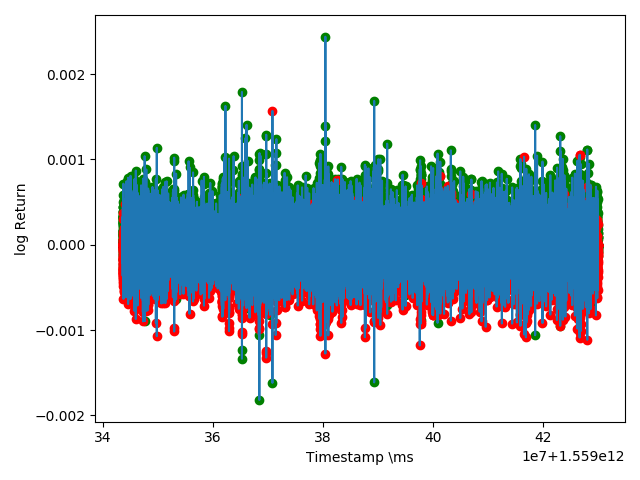
\includegraphics[width=\textwidth]{images/log_returns_per_trade}
        \caption{Whole day}
        \label{fig:log_returns}
    \end{subfigure}
    \begin{subfigure}[b]{0.45\textwidth}
        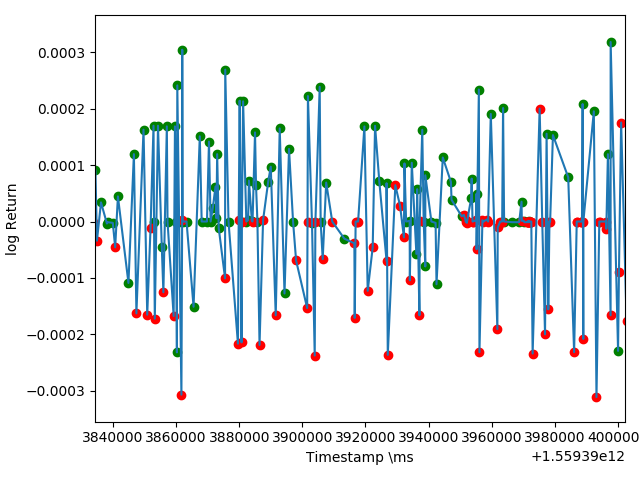
\includegraphics[width=\textwidth]{images/log_returns_per_trade_zoom}
        \caption{Typical section}
        \label{fig:log_returns_zoom}
    \end{subfigure}
    \caption{The log returns for each order on 1st July 2019. Green points represent market buy orders, red points represent market sell orders.}
    \label{log_returns}
\end{figure}
The Binomial Markov model presented in this section will serve as a base for other mode complex models. Figure \ref{log_returns} shows the log return caused by each trade, that is the logarithm of the ratio of the trade price and the previous trade price. There is a high level of dependence between the market state trades and incoming trades. To capture this, we propose a simple Markov binomial model. 
\subsection{Basic Markov Model}
We suppose that each trade either increases the log price by $\delta$ or decreases the log price by $\delta$ (we ignore trades that do not alter the price). We then assume order states (whether the order increases or decreases the price) form a Markov chain $X_i$ on the state space $\{-1, 1\}$ with transition matrix $P = (p_{ij})$ which is such that a stationary distribution exists. Let $\lambda_{ij}, i,j \in \{-1, 1\}$ be the order rate for the chain moving from state $i$ to $j$. If $V(s, n)$ is the number of visits to state $s$ before step $n$ and $\pi$ is the stationary distribution and $\sigma^2 = \sum_{i=1}^{\infty}\text{Cov}(X_0, X_i)$, then by the central limit theorem for Markov Chains \cite{markovclt}
\begin{equation}
\frac{V(s, n) - n\pi_s}{\sigma \sqrt{n}} \xrightarrow{\text{d}} \mathcal{N}(0, 1).
\end{equation}
Hence if $U_n$ ($D_n$) is the number of price increasing (decreasing) trades before time step $n$, we have that
\begin{align}
D_n = V(-1, n) &= n - V(1, n) = n - U_n \\
U_n - D_n &= 2U_n - n \\
U_n &\approx  \mathcal{N}(n\pi_1, n\sigma^2)
\end{align}
for large $n$. 
We now look at the distribution of the number of trades in a large time period, $S$. Let $T_l$ be the $l$th interarrival time (so $T_l \sim \sum \chi_{\{X_l = j, X_{l + 1} = j\}} A_{ij}^l $) where $A_{ij}^l \sim \text{Exp}(\lambda_{ij})$. So in the stationary distribution,
\begin{align}
\mathbb{E}(T_l) &= \sum_{ij} \lambda_{ij}\pi_{i}p_{ij}\\
\mathbb{E}(T_l^2) &=  \sum_{ij} 2\lambda_{ij}^2\pi_{i}p_{ij}
\end{align}
as $\pi_i p_{ij}$ is the long run proportion of jumps from state $i$ to $j$. Let $\mu = \mathbb{E}(T_l)$ and $\sigma^2 = \mathbb{E}(T_l^2) - \mathbb{E}(T_l)^2$ then if $N$ is the number of trades from time $0$ to $S$,
\begin{equation}
\mathbb{P}(N \leq n) = \mathbb{P}\left(\sum_{l=1}^n T_l \leq S\right) = \mathbb{P}\left(\frac{\sum_{l=1}^n T_l - n\mu}{\sigma \sqrt{n}} \leq \frac{S - n\mu}{\sigma \sqrt{n}} \right) 
\end{equation}
By the central limit theorem, 
\begin{equation}
\frac{\sum_{l=1}^n T_l - n\mu}{\sigma \sqrt{n}} \xrightarrow{d} \mathcal{N}(0, 1)
\end{equation}
Hence,
\begin{equation}
\mathbb{P}(N \leq n) \approx \Phi\left(\frac{S - n\mu}{\sigma \sqrt{n}} \right)
\end{equation}
for large $S$. If $R_S$ is the log return after time $S$, it follows that
\begin{equation}
\mathbb{P}\left(R_S \leq \frac{\alpha}{\delta}\right) = \sum_{n=1}^{\infty} \mathbb{P}\left(U_n - D_n \leq \alpha\right)\mathbb{P}(N = n)
\end{equation}
which is easily approximated using the derived normal approximations.
\subsection{Parameter Estimation, Generation and Evaluation of Forecasts}
The basic Markov model, for day $t$, is parametrized by the order rates ($\lambda_{i j}^t$), the transition probabilities ($p_{-1-1}^t, p_{11}^t$) and the mean change in the price caused by each trade $\delta^t$. To produce a forecast, these parameters need to be estimated and we propose this is done using linear regression on a transformed parameter time series. Let $\sigma(t) = \frac{1}{1 + e^{-x}}$ be the standard sigmoid function and let $\theta_t = (\sigma^{-1}(p_{-1-1}^t), \sigma^{-1}(p_{11}^t), \log\delta^t, \log\lambda^t)$ and then we fit the model
\begin{equation}
\theta_t = M (\theta_i)_{i=t - k}^{i=t-1} + \epsilon_t 
\end{equation}
where $M$ is a $k \times 4$ matrix and the $\epsilon_t$ are I.I.D. with a multivariate normal distribution. An interesting question is how much weight the prediction of these parameters has on the forecast. The transformation is performed to make sure that the predicted values from the time series can then be used to give meaningful results. For example, probabilities between $0$ and $1$ and positive rates and absolute value price increases.
\subsubsection{Trade Mean and Order Rates Through Time}
\begin{figure}[h]
    \centering
    \begin{subfigure}[b]{0.4\textwidth}
        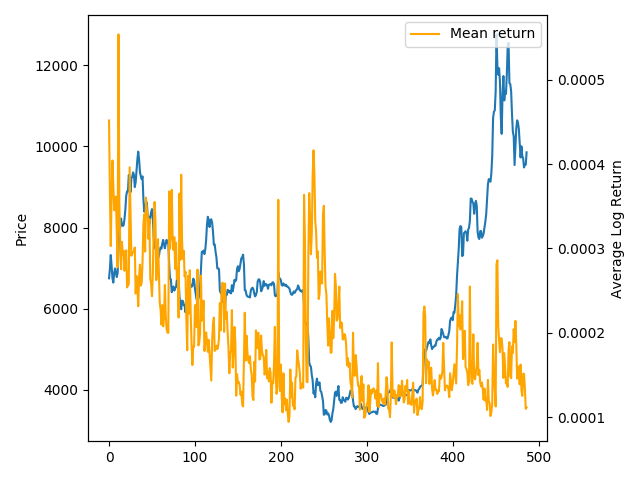
\includegraphics[width=\textwidth]{images/return_params}
        \caption{$\delta^t$}
    \end{subfigure}
    \begin{subfigure}[b]{0.4\textwidth}
        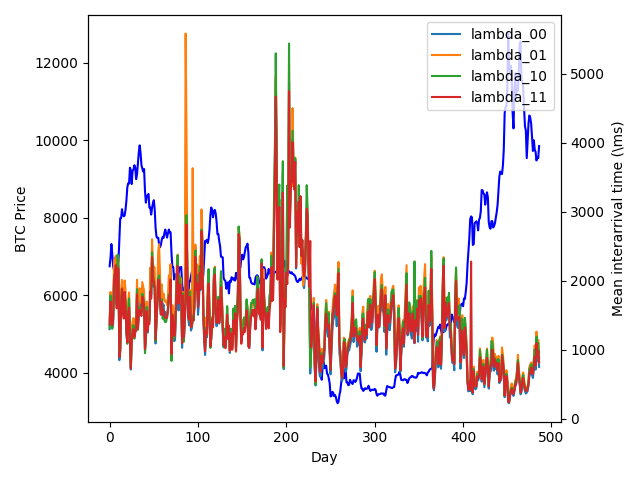
\includegraphics[width=\textwidth]{images/rate_params}
        \caption{$\lambda_{ij}^t$}
        \label{fig:log_returns_zoom}
    \end{subfigure}
    \begin{subfigure}[b]{0.4\textwidth}
        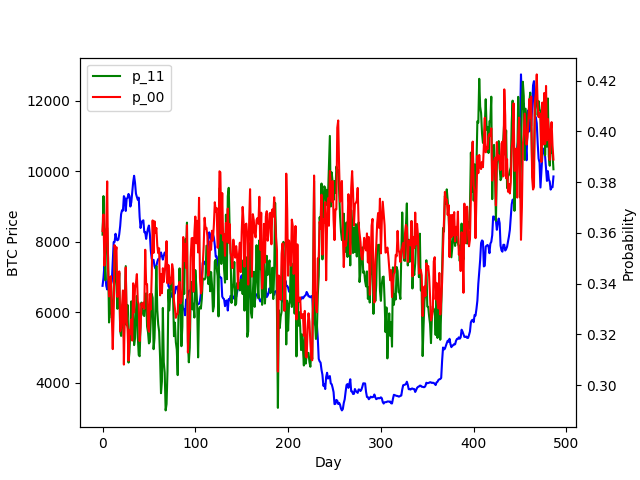
\includegraphics[width=\textwidth]{images/prob_params}
        \caption{$p_{-1-1}^t$ and $p_{11}^t$}
    \end{subfigure}
    \caption{Daily parameter time series, plotted from 1st April 2018 for 500 days. Bitcoin price is shown behind for reference.}
    \label{parameter_timeseries}
\end{figure}
\subsubsection{Evaluation of parameter prediction}
\subsection{Problems with the Model}
\subsubsection{Markov Property}
Under the null hypothesis that the process is Markovian 
\begin{equation}
\mathbb{E}\left(f(X_i) | X_{i-1}, ... ,X_{i - k}\right) = \mathbb{E}\left(f(X_i) | X_{i-1}\right) \ \forall i > 0, k < i
\end{equation}
and so to test whether this holds we plot the conditional expectations of $X_i$ where $X_i = 0$ if the $i$th trade decreases the price and $X_i = 1$ if the $i$th trade increases the price. We now show that order trades are not Markovian.  
\begin{figure}[h]
    \centering
    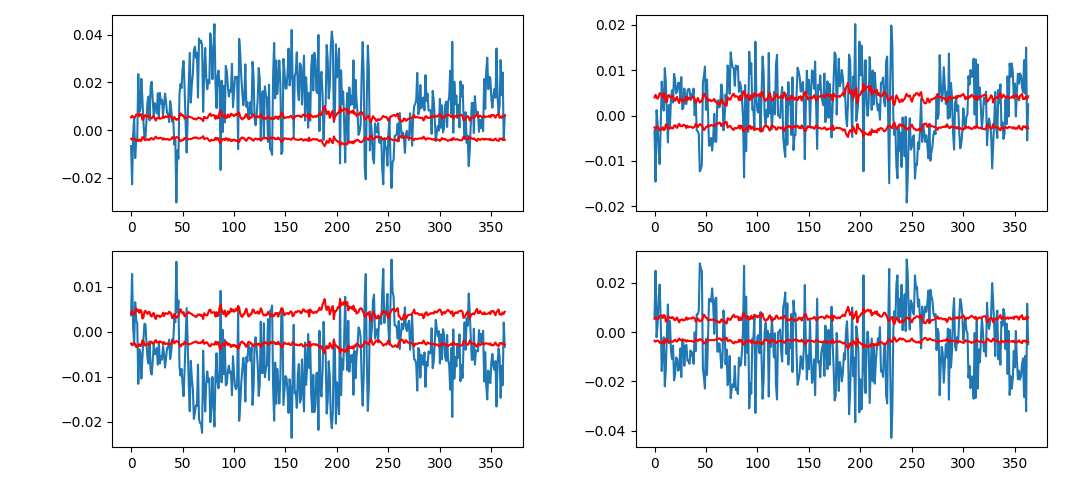
\includegraphics[width=0.6\textwidth]{images/markov95}
    \caption{Plots of $\mathbb{E}(X_i | X_{i-1}, X_{i-2}) - \mathbb{E}(X_i | X_{i-1})$ with $95\%$ confidence interval shown for each day assuming no dependence on $X_{i - 2}$. In clockwise order, the state values are $(X_{i - 2} = 0, X_{i - 1} = 0), (X_{i - 2} = 1, X_{i - 1} = 0), (X_{i - 2} = 0, X_{i - 1} = 1), (X_{i - 2} = 1, X_{i - 1} = 1)$}
    \label{CI95markov}
\end{figure}
Figure \ref{CI95markov} shows a clear rejection of the Markov hypothesis, indicating that information is missing under the assumption. A similar analysis in Figure \ref{CI952ndordermarkov}. Looking at $\mathbb{E}(X_i | X_{i-1}. X_{i - 2}, X_{i-3}) - \mathbb{E}(X_i | X_{i-1}. X_{i - 2})$ indicates that after two consecutive orders in the same direction, there is a much higher chance of a reversal order than given under the Markov hypothesis, indicating that trades tend to try and undo price changes. Section \ref{markovreplacement} suggests a way to improve this.
\begin{figure}[h]
    \centering
    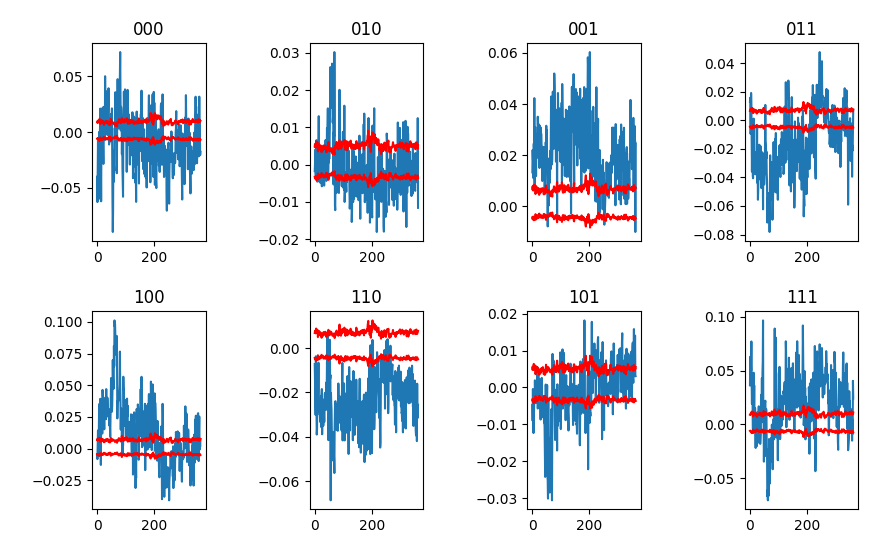
\includegraphics[width=0.7\textwidth]{images/2ndordermarkov}
    \caption{Plots of $\mathbb{E}(X_i | X_{i-1}, X_{i-2}, X_{i-3}) - \mathbb{E}(X_i | X_{i-1}, X_{i - 2})$ with $95\%$ confidence interval shown for each day assuming that there is no dependence on $X_{i-3}$. The titles of each plot give the state of the chain.}
    \label{CI952ndordermarkov}
\end{figure}
\subsubsection{Exponential Order Rates}
In general the complete order interarrival times (not ignoring trades that alter the price) form a Weibull$(\alpha, \beta)$ distribution (a distribution with cumulative distribution function $F_{\alpha,\beta}(x) = 1 - e^{\alpha x^\beta}$), which we assume is due to a process which is more or less exponentially distributed (independent retail investor trades, for example) and then with some reactions which lead to a order rate function that depends on orders occurring. This analysis is left to the appendix.
\section{Model Improvements}
We now address the issues with the basic Markov model shown in the statistical analysis.
\subsection{Markov Property}
\label{markovreplacement}
Figure \ref{CI95markov} shows that the direction of the next order depends on the history of the chain as well as the current state. Figure \ref{CI952ndordermarkov} suggests that the proportion of previous price increasing trades can be used to determine whether the markov model over or under predicts the probability of the next trade increasing the price. To investigate this we introduce an exponential moving average (EMA) of the trade property as follows. If $X_i$ is defined as above, let the EMA $S_i$ be such that
\begin{align}
S_1 &= X_1 \\
S_i &= \alpha X_i + (1 - \alpha)S_{i-1}
\end{align}
for $\alpha \in (0, 1)$. We wish to calculate the marginal expectation $\mathbb{E}(X_i | S_{i-1})$. Noting that $\mathbb{E}(X_i | S_{i-1} \leq s) = \mathbb{P}(X_i = 1 | S_{i-1} \leq s)$ and using Bayes' theorem we have that
\begin{equation}
\mathbb{E}(X_i | S_{i-1} \leq s) = \frac{\mathbb{P}(S_{i-1} \leq s | X_i = 1)\mathbb{P}(X_i = 1)}{\mathbb{P}(S_{i-1} \leq s)}
\end{equation}
which can be computed empirically from the data. Now let $f(s) = \mathbb{E}(X_i | S_{i-1} \leq s)$, $p(s) = \mathbb{E}(X_i | S_{i-1} = s)$ and $\mu(s)$ be the probability law defined by $S_i$. Then (TODO sort out notation for this)
\begin{align}
f(x) &= \frac{\int_0^x p(t)d\mu(t)}{\int_0^x d\mu} \\
\Rightarrow p(x) &= \frac{df}{d\mu}(x)\int_0^xd\mu + f(x)
\end{align}
which can then be calculated empirically from the data, this is shown in Figure \ref{probgivenema}.
\begin{figure}[h]
    \centering
    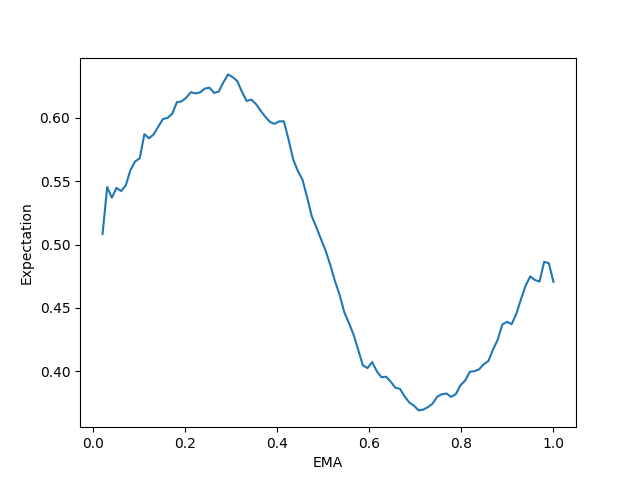
\includegraphics[width=0.4\textwidth]{images/conditional_expectation1}
    \caption{$p(x)$ (Expectation) against $x$ (EMA), $\alpha = 0.3$}
    \label{probgivenema}
\end{figure}
\subsubsection{Statistical Analysis}
After deriving this result we now show that the EMA method is an effective way to predict market movements, drastically improving the forecasting accuracy of the basic Markov model. To do this we calculate the Brier Score for the next trade forecasts calculated using the EMA. A difficulty in evaluating the performance of the EMA method for forecasting the next trade, as with evaluating any forecast, is to know whether a better forecasting technique exists. We compare against a neural network to see if the moving average trade is likely capturing relevant information.
\subsection{Parameter Price Dependence}
\section{Appendix}
\subsection{Portfolio Selection}
\subsection{Order Interarrivals}
\medskip
\printbibliography

\end{document}